\documentclass[12pt,a4paper]{article}
\usepackage[utf8]{inputenc}
\usepackage[portuguese]{babel}
\usepackage{amsmath}
\usepackage{graphicx}
\usepackage{geometry}
\geometry{a4paper, margin=2.5cm}
\usepackage{hyperref}
\usepackage{float}
\usepackage{tikz}
\usetikzlibrary{shapes.geometric, arrows.meta, positioning}

\begin{document}

% ==========================================
% CAPA DO RELATÓRIO
% ==========================================
\begin{titlepage}
    \begin{center}
        
\includegraphics[width=5cm]{images/logo_uminho.png}

        \vspace{1cm}
        {\Huge \textbf{Projeto CG}} \\[0.4cm]
        {\large Grupo TP-06} \\[0.2cm]
        {\large Universidade do Minho} \\
        {\large Licenciatura em Engenharia Informática} \\
        {\large Computação Gráfica - 2025/26}
        \vspace{1.5cm}

        \vspace{1.5cm}

        \begin{minipage}{0.23\textwidth}
            \centering
            
\includegraphics[width=3cm,height=3cm]{images/foto_goncalo.jpeg} \\
            Gonçalo Costa \\ \texttt{A107381}
        \end{minipage}
        \hspace{0.5cm}
        \begin{minipage}{0.23\textwidth}
            \centering
            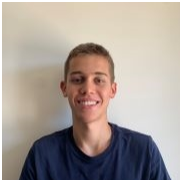
\includegraphics[width=3cm,height=3cm]{images/foto_diogo.jpeg} \\
            Diogo Costa \\ \texttt{A107328}
        \end{minipage}
        \hspace{0.5cm}
        \begin{minipage}{0.23\textwidth}
            \centering
            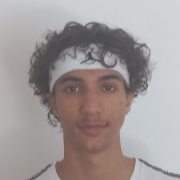
\includegraphics[width=3cm,height=3cm]{images/foto_lourenco.jpeg} \\
            Lourenço Martins \\ \texttt{A106849}
        \end{minipage}
        \hspace{0.5cm}
        \begin{minipage}{0.23\textwidth}
            \centering
            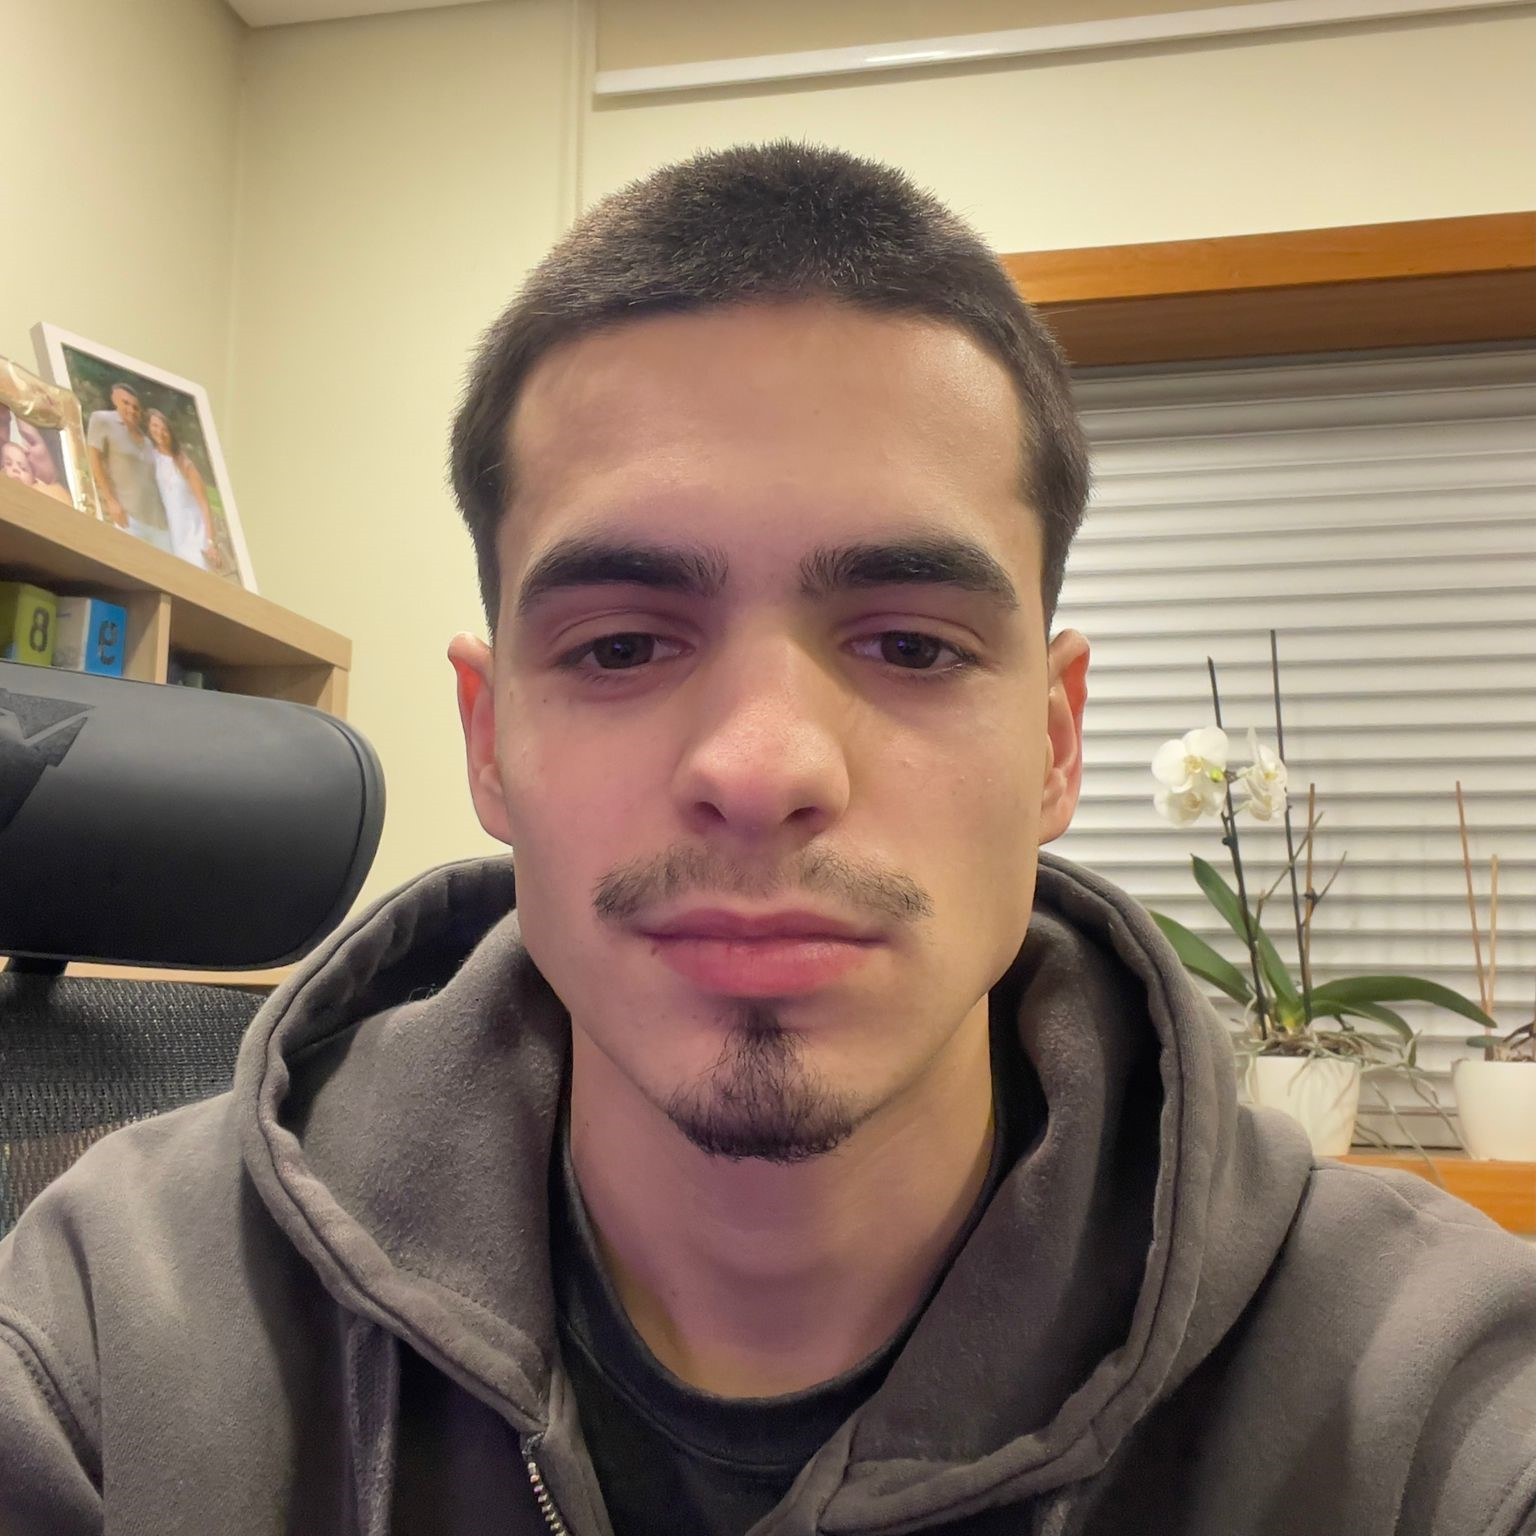
\includegraphics[width=3cm,height=3cm]{images/foto_sa.jpeg} \\
            Gonçalo Sá \\ \texttt{A107376}
        \end{minipage}

        \vfill
        \textbf{29 de abril de 2026}
    \end{center}
\end{titlepage}

\tableofcontents
\newpage

% ==========================================
% 1. INTRODUÇÃO
% ==========================================
\section{Introdução}

O presente relatório detalha o desenvolvimento da terceira fase do projeto da unidade curricular de Computação Gráfica. Esta fase acrescentou duas grandes funcionalidades ao trabalho já realizado: a capacidade do \textit{Generator} produzir modelos baseados em \textit{patches} de Bézier, e a capacidade do \textit{Engine} suportar transformações geométricas animadas e renderização com \textit{Vertex Buffer Objects} (VBOs).

As animações assentam em dois mecanismos: rotações controladas por um período de tempo e translações dirigidas por curvas de Catmull-Rom, com suporte ao alinhamento do objeto com a tangente da curva. A cena de demonstração é um sistema solar dinâmico com todos os planetas, a Lua da Terra, os anéis de Saturno e dois cometas construídos com \textit{patches} de Bézier.

% ==========================================
% 2. GENERATOR
% ==========================================
\section{Generator}

\subsection{Construção de modelos com \textit{patches} de Bézier}

O \textit{Generator} foi expandido com o comando \texttt{patch}, que recebe um ficheiro \texttt{.patch}, o nível de tessellação e o ficheiro de saída. O formato do ficheiro segue a especificação fornecida: a primeira linha contém o número de \textit{patches}; seguem-se os 16 índices de pontos de controlo de cada \textit{patch} separados por vírgulas; depois o número total de pontos de controlo e as suas coordenadas $(x, y, z)$.

\subsubsection{Fórmula da superfície de Bézier}

Cada ponto da superfície é calculado através dos polinómios de Bernstein de grau 3. Dados os parâmetros $(u, v) \in [0,1]^2$, o ponto resultante é:

\begin{equation}
    \mathbf{p}(u,v) = \sum_{i=0}^{3} \sum_{j=0}^{3} B_i(u)\, B_j(v)\, \mathbf{P}_{ij}
\end{equation}

onde $\mathbf{P}_{ij}$ são os 16 pontos de controlo do \textit{patch} e $B_k(t)$ são os polinómios de Bernstein:

\begin{equation}
    B_0(t) = (1-t)^3, \quad
    B_1(t) = 3t(1-t)^2, \quad
    B_2(t) = 3t^2(1-t), \quad
    B_3(t) = t^3
\end{equation}

\subsubsection{Tessellação e triangulação}

Para cada \textit{patch}, a superfície é amostrada numa grelha $T \times T$ (onde $T$ é o nível de tessellação). Para cada célula $(i,j)$ da grelha, calculam-se quatro cantos com os parâmetros:

\begin{equation}
    \text{P1} = \left(\tfrac{i}{T},\, \tfrac{j}{T}\right), \quad
    \text{P2} = \left(\tfrac{i+1}{T},\, \tfrac{j}{T}\right), \quad
    \text{P3} = \left(\tfrac{i+1}{T},\, \tfrac{j+1}{T}\right), \quad
    \text{P4} = \left(\tfrac{i}{T},\, \tfrac{j+1}{T}\right)
\end{equation}

Os quatro cantos são divididos em dois triângulos — (P1, P4, P2) e (P2, P4, P3) — respeitando a \textit{winding order} para que as normais apontem para o exterior.

% ==========================================
% 3. ENGINE
% ==========================================
\section{Engine}

\subsection{Alterações às estruturas de dados}

Para suportar as transformações animadas foram adicionados três campos à estrutura \textit{Transform}:

\begin{itemize}
    \item \textbf{time} — período em segundos para uma rotação completa ou para percorrer toda a curva;
    \item \textbf{align} — indica se o objeto deve orientar-se com a tangente da curva (exclusivo da translação animada);
    \item \textbf{points} — vetor de pontos de controlo da curva de Catmull-Rom.
\end{itemize}

Foi também criada a estrutura \textit{ModelVBO}, que armazena o identificador do \textit{buffer} na GPU (\texttt{vbo\_id}) e o número de vértices (\texttt{vert\_count}), substituindo o envio de vértices em modo imediato.

\subsection{Rotações dependentes do tempo}

O elemento XML \texttt{<rotate>} pode agora receber o atributo \texttt{time} em vez de \texttt{angle}. Em cada \textit{frame}, o ângulo de rotação é calculado a partir do tempo decorrido, obtido com \texttt{glutGet(GLUT\_ELAPSED\_TIME)}:

\begin{equation}
    \alpha(t) = \frac{t}{t_r} \times 360°
    \label{eq:rotacao}
\end{equation}

onde $t$ é o tempo decorrido em segundos e $t_r$ o período definido no XML. Se o atributo \texttt{time} não estiver presente, a rotação é estática e usa o valor de \texttt{angle}.

\subsection{Translações dirigidas por curvas de Catmull-Rom}

O elemento \texttt{<translate>} pode agora receber os atributos \texttt{time} e \texttt{align}, e um conjunto de pontos filhos \texttt{<point>} que definem a curva. O mínimo de 4 pontos é obrigatório pela definição da curva de Catmull-Rom.

\subsubsection{Cálculo do ponto na curva}

A função \texttt{getCatmullRomPoint} calcula um ponto dado quatro pontos de controlo consecutivos $\mathbf{P}_0, \mathbf{P}_1, \mathbf{P}_2, \mathbf{P}_3$ e um parâmetro local $t \in [0,1]$:

\begin{equation}
    \mathbf{p}(t) = \begin{bmatrix} t^3 & t^2 & t & 1 \end{bmatrix} \cdot M \cdot \begin{bmatrix} \mathbf{P}_0 \\ \mathbf{P}_1 \\ \mathbf{P}_2 \\ \mathbf{P}_3 \end{bmatrix}
    \label{eq:catmull}
\end{equation}

onde $M$ é a matriz de Catmull-Rom:

\begin{equation}
    M = \begin{bmatrix}
        -0.5 &  1.5 & -1.5 &  0.5 \\
         1.0 & -2.5 &  2.0 & -0.5 \\
        -0.5 &  0.0 &  0.5 &  0.0 \\
         0.0 &  1.0 &  0.0 &  0.0
    \end{bmatrix}
\end{equation}

A curva interpolada passa pelos pontos $\mathbf{P}_1$ e $\mathbf{P}_2$; os pontos $\mathbf{P}_0$ e $\mathbf{P}_3$ são auxiliares e controlam as tangentes nas extremidades do segmento, garantindo continuidade $C^1$ entre segmentos adjacentes — isto é, a curva é contínua e sem quebras abruptas de direção.

A derivada $\mathbf{p}'(t)$, necessária para o alinhamento, é obtida substituindo o vetor $T = [t^3\ t^2\ t\ 1]$ por $T' = [3t^2\ 2t\ 1\ 0]$ na equação~\eqref{eq:catmull}.

\subsubsection{Parametrização global}

A função \texttt{getGlobalCatmullRomPoint} recebe um parâmetro global $g_t \in [0, 1[$ que representa a posição ao longo de toda a curva fechada. O parâmetro é calculado a partir do tempo decorrido como:

\begin{equation}
    g_t = \frac{\text{fmod}(t,\, t_r)}{t_r}
\end{equation}

garantindo que $g_t$ se repete ciclicamente e a animação nunca para. O segmento e o parâmetro local são então determinados por:

\begin{equation}
    t_{\text{global}} = g_t \times N, \quad
    \text{index} = \lfloor t_{\text{global}} \rfloor, \quad
    t_{\text{local}} = t_{\text{global}} - \text{index}
\end{equation}

onde $N$ é o número de pontos de controlo. Os quatro pontos do segmento são selecionados com índices cíclicos (módulo $N$) para garantir a continuidade da curva fechada.

\subsubsection{Alinhamento com a tangente}

Quando \texttt{align="true"}, a orientação do objeto é atualizada em cada \textit{frame} para que o seu eixo $X$ aponte na direção da tangente. O sistema de eixos é construído como:

\begin{equation}
    \mathbf{X}_i = \text{normalizar}\!\left(\mathbf{p}'(t)\right), \quad
    \mathbf{Z}_i = \text{normalizar}\!\left(\mathbf{X}_i \times \mathbf{Y}_{\text{up}}\right), \quad
    \mathbf{Y}_i = \text{normalizar}\!\left(\mathbf{Z}_i \times \mathbf{X}_i\right)
\end{equation}

onde $\mathbf{Y}_{\text{up}} = (0, 1, 0)$ é o vetor de referência e $\times$ representa o produto vetorial. Os três vetores são organizados numa matriz de rotação $4 \times 4$ e aplicados com \texttt{glMultMatrixf} após a translação.

\subsection{Utilização de VBOs}

Na fase anterior, os vértices eram enviados à GPU em modo imediato em cada \textit{frame}. Nesta fase, os dados de geometria são carregados uma única vez na inicialização pela função \texttt{loadModel}:

\begin{enumerate}
    \item Leitura dos vértices do ficheiro \texttt{.3d} para um vetor de \textit{floats} no formato $[x, y, z, x, y, z, \ldots]$;
    \item Geração de um \textit{buffer} com \texttt{glGenBuffers} e ativação com \texttt{glBindBuffer};
    \item Transferência dos dados para a GPU com \texttt{glBufferData(GL\_STATIC\_DRAW)};
    \item Armazenamento do identificador e da contagem de vértices na estrutura \textit{ModelVBO}.
\end{enumerate}

Durante a renderização, a função \texttt{drawGroup} usa \texttt{glBindBuffer}, \texttt{glVertexPointer} e \texttt{glDrawArrays(GL\_TRIANGLES)} para cada modelo. O estado \texttt{GL\_VERTEX\_ARRAY} é ativado uma única vez no arranque com \texttt{glEnableClientState}. Uma garantia importante desta abordagem é que o carregamento dos buffers ocorre durante o \textit{parsing} do XML, percorrendo a árvore de grupos pela mesma ordem que a renderização — assim, cada \texttt{vbo\_id} armazenado na estrutura \textit{ModelVBO} corresponde sempre ao modelo correto no momento do desenho.

\subsection{Câmara esférica orbital}

A câmara implementada assenta em coordenadas esféricas e foca-se num ponto alvo móvel (\textit{lookAt}). O utilizador pode orbitar em torno desse ponto com o botão esquerdo do rato (altera os ângulos $\alpha$ e $\beta$), fazer \textit{zoom} com o botão direito (altera o raio $r$), e deslocar o ponto alvo com as setas direcionais e as teclas \texttt{w}/\texttt{s}. A posição da câmara é recalculada em cada interação através das equações de conversão esférica-cartesiana:

\begin{equation}
    \text{camX} = \text{lookX} + r\,\sin(\alpha)\cos(\beta), \quad
    \text{camY} = \text{lookY} + r\,\sin(\beta), \quad
    \text{camZ} = \text{lookZ} + r\,\cos(\alpha)\cos(\beta)
\end{equation}

Os ângulos iniciais $\alpha$ e $\beta$ e o raio $r$ são calculados automaticamente a partir das posições \texttt{position} e \texttt{lookAt} lidas do XML, pelo que a câmara parte sempre da perspetiva definida na configuração. O ângulo $\beta$ é restrito ao intervalo $[-85°, 85°]$ para evitar a inversão da perspetiva no polo.

% ==========================================
% 4. SISTEMA SOLAR E EXTRAS
% ==========================================
\section{Sistema Solar e Extras}

\subsection{Visão geral}

A cena de demonstração inclui o Sol, todos os planetas do sistema solar, a Lua da Terra, os anéis de Saturno e dois cometas. Todos os movimentos orbitais e as rotações axiais são animados e dependentes do tempo. A hierarquia de grupos XML garante que os corpos dependentes (Lua, anéis de Saturno) herdam corretamente as transformações dos seus grupos pai.

No ficheiro XML, cada planeta é um grupo independente ao mesmo nível — não existem relações de pai/filho entre planetas. As únicas hierarquias reais presentes na cena são duas: a Lua como subgrupo da Terra, e os anéis de Saturno como subgrupo de Saturno. Graças ao isolamento de matrizes com \texttt{glPushMatrix}/\texttt{glPopMatrix}, cada subgrupo herda automaticamente a translação orbital do seu pai.

\begin{figure}[H]
    \centering
    \begin{tikzpicture}[
        node distance=1.4cm and 2cm,
        group/.style={draw=blue!60, rectangle, rounded corners, minimum width=3cm, minimum height=0.8cm, align=center, fill=blue!5, font=\sffamily\bfseries},
        model/.style={draw=green!60!black, rectangle, rounded corners, minimum width=2.6cm, minimum height=0.6cm, align=center, fill=green!5, font=\sffamily\footnotesize},
        arrow/.style={-{Stealth[scale=1.2]}, thick, draw=gray!80},
        lbl/.style={font=\footnotesize\itshape, text=blue!80!black, align=right}
    ]
        % --- Hierarquia Terra-Lua ---
        \node[group] (terra) at (0, 0)    {Group (Terra)};
        \node[model] (mterra) at (3.2, 0) {Esfera (Terra)};
        \draw[arrow] (terra) -- (mterra);

        \node[group] (lua) at (0, -1.8)   {Group (Lua)};
        \node[model] (mlua) at (3.2, -1.8){Esfera (Lua)};
        \draw[arrow] (lua) -- (mlua);

        \draw[arrow, draw=blue!60] (terra.south) -- (lua.north)
            node[midway, left=4pt, lbl]{Translação CR};

        % --- Hierarquia Saturno-Anéis ---
        \node[group] (saturno) at (7.5, 0)    {Group (Saturno)};
        \node[model] (msat)    at (10.7, 0)   {Esfera (Saturno)};
        \draw[arrow] (saturno) -- (msat);

        \node[group] (aneis) at (7.5, -1.8)   {Group (Anéis)};
        \node[model] (maneis) at (10.7, -1.8) {Torus (Anéis)};
        \draw[arrow] (aneis) -- (maneis);

        \draw[arrow, draw=blue!60] (saturno.south) -- (aneis.north)
            node[midway, left=4pt, lbl]{Escala};

    \end{tikzpicture}
    \caption{As duas hierarquias de grupos presentes na cena. À esquerda: a Lua orbita a Terra como subgrupo, herdando a sua translação orbital. À direita: os anéis de Saturno acompanham o planeta como subgrupo, com uma escala aplicada para os achatar.}
    \label{fig:grafo_solar}
\end{figure}

\subsection{Cometas com \textit{patches} de Bézier}

O enunciado requeria pelo menos um cometa construído com \textit{patches} de Bézier e trajetória de Catmull-Rom. Foram implementados dois:

\begin{itemize}
    \item \textbf{Cometa 1} — órbita excêntrica e inclinada relativamente ao plano $XZ$, com \texttt{align="true"} para que o objeto se oriente com a tangente em cada instante. A sua geometria é definida por \texttt{comet.patch}, composto por 6 \textit{patches} de Bézier. Os 3 primeiros formam a superfície lateral cônica: os 4 pontos de controlo do topo convergem todos para o mesmo ponto $(0, 0, 3)$, forçando a superfície a afunilar numa ponta, enquanto a base se abre para um raio de 1 unidade em $z=0$. Os 3 \textit{patches} restantes fecham a superfície pelo lado da base, sendo construídos com os índices dos primeiros transpostos para inverter a \textit{winding order} e garantir normais coerentes em toda a superfície.
    \item \textbf{Cometa 2} — órbita circular de raio muito superior ao dos planetas exteriores, simulando um cometa de longo período que percorre regiões afastadas do sistema solar.
\end{itemize}

\subsection{Extras de realismo astronómico}

Para além dos requisitos mínimos, foram introduzidos vários detalhes de precisão astronómica:

\begin{itemize}
    \item \textbf{Urano com inclinação axial de $\sim$98°} — O eixo de rotação foi definido como quase horizontal (\texttt{x="0.99" y="0.1" z="0"}), fazendo Urano rolar ao longo da sua órbita, tal como acontece na realidade.

    \item \textbf{Vénus com rotação retrógrada} — O sentido de rotação foi invertido (\texttt{y="-1"}), reproduzindo a rotação retrógrada de Vénus. O período de 60 segundos reflete também o seu dia solar extremamente longo.

    \item \textbf{Mercúrio com órbita excêntrica} — A curva de Catmull-Rom de Mercúrio é assimétrica: o afélio está a $x=24$ e o periélio a $x=-18$, gerando uma elipse achatada que simula a maior excentricidade orbital do sistema solar ($e \approx 0.21$).

    \item \textbf{Lua com inclinação orbital} — Os pontos de controlo da órbita da Lua têm coordenadas $y$ não nulas ($y=\pm 0.5$ em pontos alternados), reproduzindo a inclinação de $\sim$5° da órbita lunar em relação à eclíptica.

    \item \textbf{Anéis de Saturno em hierarquia correta} — O torus dos anéis é grupo filho de Saturno, acompanhando-o automaticamente na sua órbita. A escala $(5.5, 0.15, 5.5)$ achata o torus para simular a geometria real dos anéis.
\end{itemize}

\subsection{Resultado final}

% --- Imagens do sistema solar ---
\begin{figure}[H]
    \centering
    \begin{minipage}{0.48\textwidth}
        \centering
        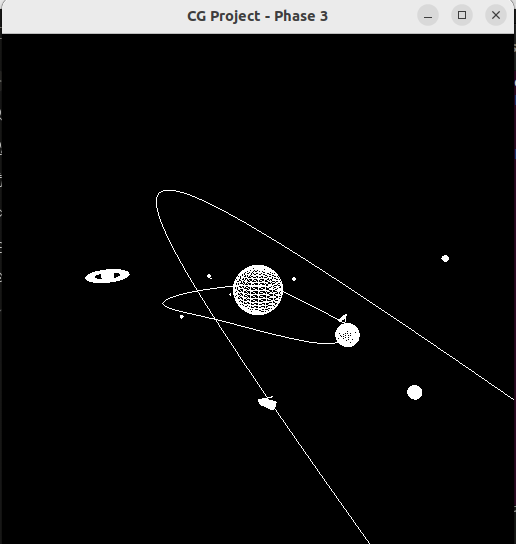
\includegraphics[width=\textwidth]{images/sistema_solar_fase3.png}
        \caption{Visão global do sistema solar animado em modo \textit{wireframe}.}
        \label{fig:solar_geral}
    \end{minipage}\hfill
    \begin{minipage}{0.48\textwidth}
        \centering
        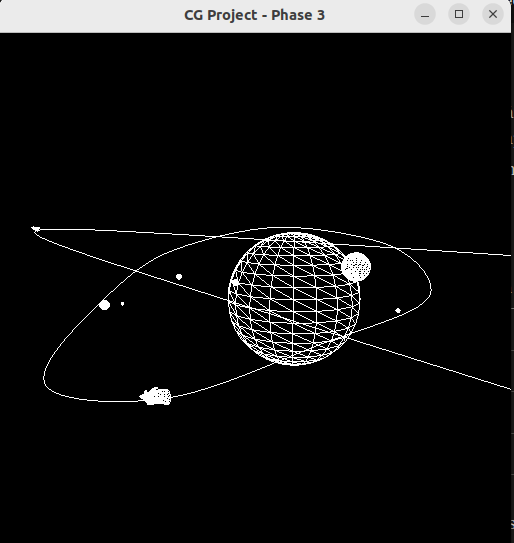
\includegraphics[width=\textwidth]{images/cometas_orbitas.png}
        \caption{Sistema solar com as trajetórias dos dois cometas visíveis.}
        \label{fig:cometas}
    \end{minipage}
\end{figure}

\begin{figure}[H]
    \centering
    \begin{minipage}{0.48\textwidth}
        \centering
        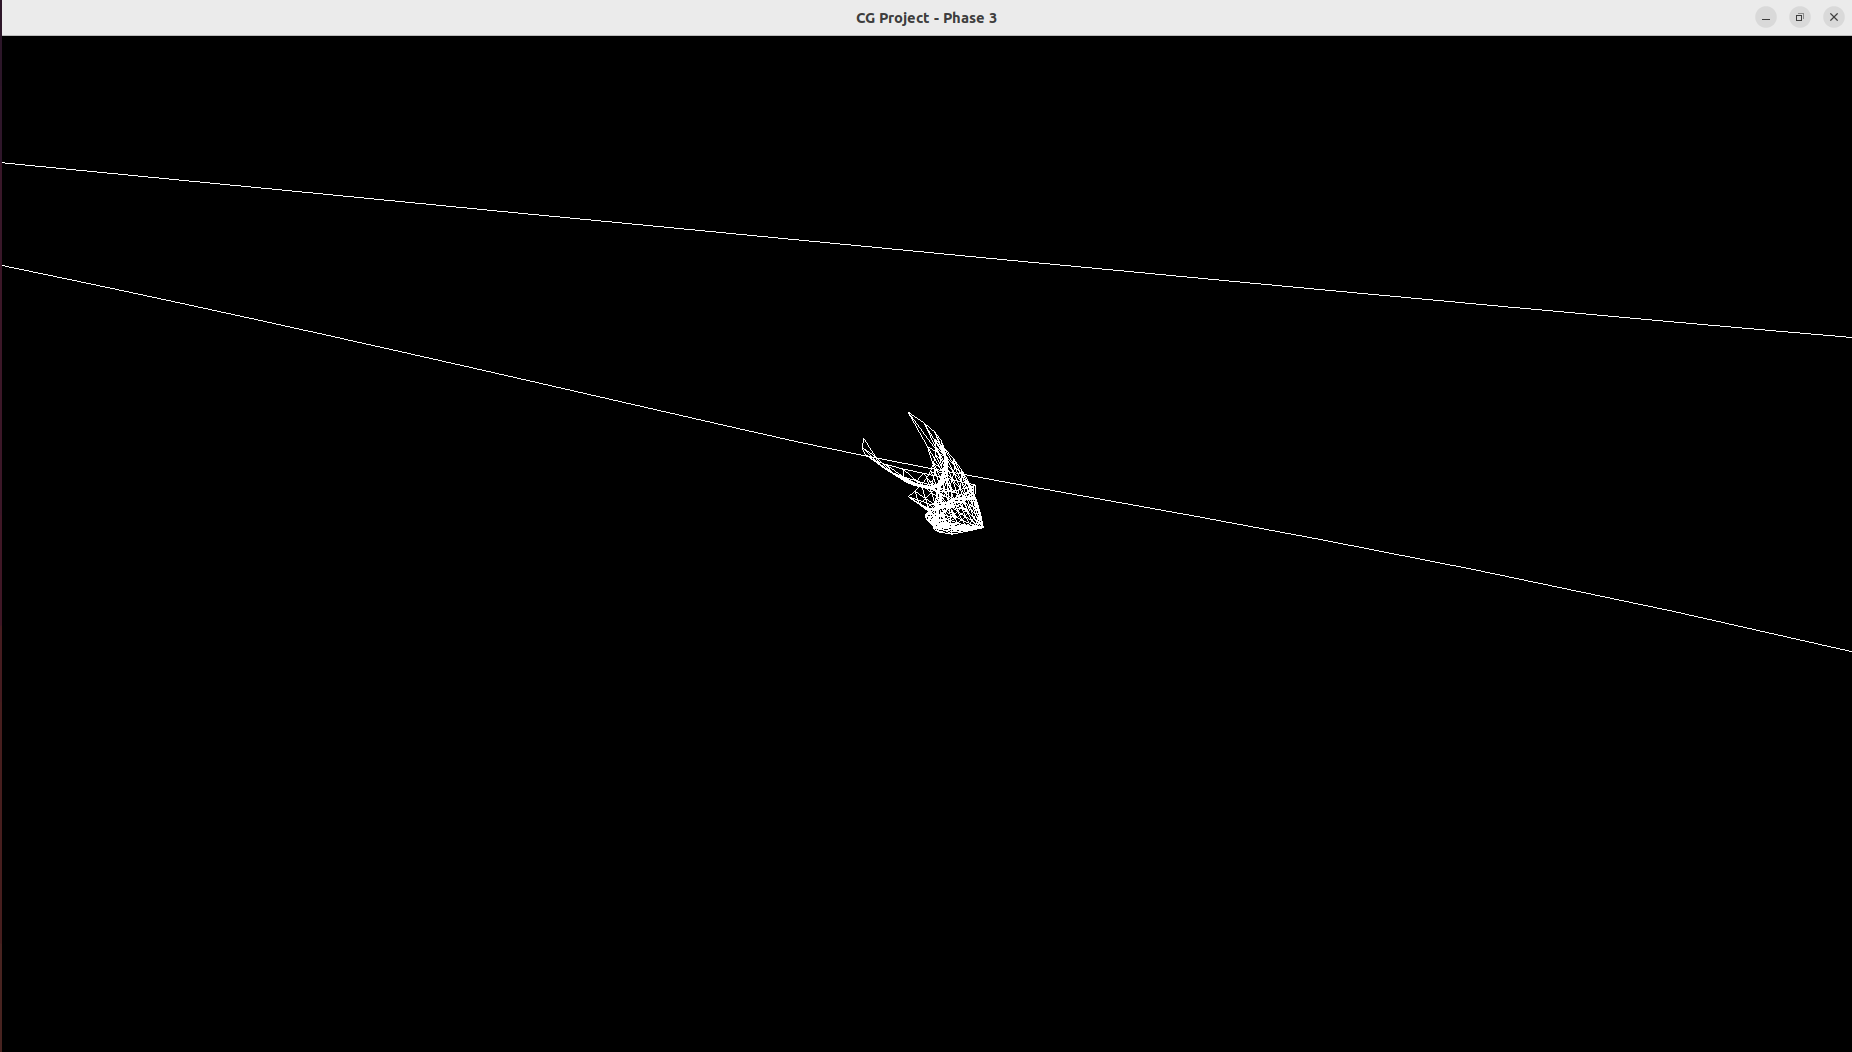
\includegraphics[width=\textwidth]{images/cometa_detalhe.png}
        \caption{Detalhe do cometa 1 construído com \textit{patches} de Bézier, alinhado com a tangente da curva de Catmull-Rom.}
        \label{fig:cometa_detalhe}
    \end{minipage}\hfill
    \begin{minipage}{0.48\textwidth}
        \centering
        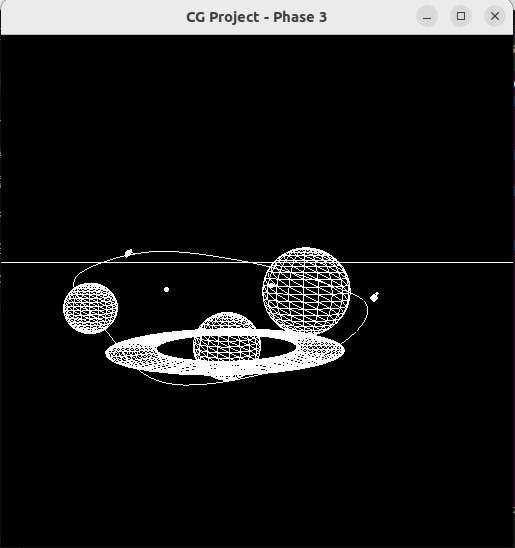
\includegraphics[width=\textwidth]{images/saturno_fase3.png}
        \caption{Detalhe de Saturno com os anéis (torus) a acompanhar o planeta na sua órbita.}
        \label{fig:saturno_f3}
    \end{minipage}
\end{figure}

% ==========================================
% 5. TESTES
% ==========================================
\section{Testes}

Antes da elaboração da cena final, a correção das funcionalidades implementadas foi validada com dois cenários de teste fornecidos.

O \textbf{Teste 1} valida em simultâneo a translação animada por curva de Catmull-Rom com alinhamento e a rotação animada em grupos hierárquicos. O ficheiro XML define um grupo pai com rotação animada (\texttt{time="3"} em torno do eixo Y) e um grupo filho cujo modelo (\texttt{bezier\_10.3d}) percorre uma curva fechada de 4 pontos com \texttt{align="true"}, uma rotação estática de $-90°$ no eixo X e uma escala de 0.5. O resultado esperado é o teapot a mover-se ao longo da órbita orientando-se com a tangente da curva, enquanto toda a cena roda em torno da origem.

O \textbf{Teste 2} valida a geração de modelos com \textit{patches} de Bézier e a sua renderização com VBOs. O ficheiro XML carrega o modelo \texttt{bezier\_10.3d} (gerado a partir de \texttt{teapot.patch} com tessellação 10) com uma rotação estática de $-90°$ no eixo X. O resultado esperado é o teapot estático corretamente posicionado e com a geometria bem formada.

\begin{figure}[H]
    \centering
    \begin{minipage}{0.48\textwidth}
        \centering
        
\includegraphics[width=\textwidth]{images/test_3_1.png}
        \caption{Teste 1: teapot a percorrer a curva de Catmull-Rom com \texttt{align="true"}, dentro de um grupo com rotação animada.}
        \label{fig:teste1}
    \end{minipage}\hfill
    \begin{minipage}{0.48\textwidth}
        \centering
        
\includegraphics[width=\textwidth]{images/test_3_2.png}
        \caption{Teste 2: teapot gerado a partir de \textit{patches} de Bézier com tessellação 10, renderizado com VBOs.}
        \label{fig:teste2}
    \end{minipage}
\end{figure}

% ==========================================
% 6. CONCLUSÃO
% ==========================================
\section{Conclusão}

Ao longo desta terceira fase, foram implementados com sucesso todos os requisitos do enunciado: geração de modelos com \textit{patches} de Bézier, translações animadas por curvas de Catmull-Rom com suporte a alinhamento, rotações dependentes do tempo e renderização com VBOs.

A migração para VBOs elimina o reenvio de vértices em cada \textit{frame}, transferindo os dados de geometria para a memória da GPU durante a inicialização, com ganhos de desempenho proporcionais ao número de polígonos da cena. A curva de Catmull-Rom permitiu criar trajetórias suaves e contínuas para os corpos celestes, e os \textit{patches} de Bézier abriram a possibilidade de modelar formas orgânicas de forma paramétrica.

Para além dos requisitos mínimos, foram introduzidos detalhes de realismo astronómico que enriquecem a cena: a inclinação axial de Urano, a rotação retrógrada de Vénus, a órbita excêntrica de Mercúrio, a inclinação da órbita da Lua e dois cometas com geometrias e órbitas distintas. O grupo considera o trabalho desta fase concluído com sucesso e a base preparada para a fase seguinte, que introduzirá iluminação, normais e texturas.

\end{document}